\section{Introduction}
\subsection{Purpose of this project}
    In this project, we implemented a system that allows the user to paint on the screen using intuitive gestures instead of the mouse. 
    Instead of using any specific draw pad or other device, we will implement the system using a simple white paper, a web cam, and a light source. 
    Without any tactile input, we are going to rely on visual inputs to determine the gesture and the position of user's hand in real-time. 
    The challenging part about this project is how to define the natural gestures that human use to indicate the drawing on a  blank paper, and how to recognize them using pure visual signal processing. Because the system only rely on the visual input, this project is perfectly suitable as an example of a visual interface. 
\subsection{Previous work}
    EnhancedDesk\cite{a} is a two handed drawing system using infrared camera. Left hand and right hand have the different role.  Isard, Michael, and John MacCormick implemented a vision based drawing package to demonstrate the hand tracking method\cite{b}.
\subsection{Program features}
The user will be given a device that consists of a white paper, a webcam that looks down from above, 
and a light source that projects light onto the paper from a non-perpendicular angle.
The distance between the webcam and the paper, the paper and the light source, and the angle of the light source are all fixed. On the bottom of the paper are some color blocks which represent a palette, and possibly some symbols which represent the drawing tools that the user can choose. The user can simply touch the color blocks to choose the color, and touch the tool symbols to choose the painting tool he or she wants to use. On the same time there will be a program on the computer screen which shows the canvas on which the user draws. 
To draw a picture, the user can use the most intuitive gesture -- use the index finger like a pen. 
Touching the paper with the index finger means to draw, while moving the finger without touching the paper means to move the pen without drawing. 
This gesture, when the user touches the palette or the symbols instead of the empty area, means to select the color or the tool instead of drawing. 
For convenience, we will also define an erase gesture, which is a palm facing downwards with the four fingers stretching straight. This gesture is easy to use, and suitable for the semantic of erase, because it is the movement one will use to wipe something away from a surface.
\subsection{Domain engineering}
Fig.\ref{fig:1} shows the setting of our device. The height from the camera to the paper canvas is 54 cm. The camera looks down so that we can convert the coordinate of the fingertip to the canvas coordinate easily. The canvas on the paper is 19cm by 14cm. We set all of back ground as white in order to detect hands easily. We use the web cam, logicool carl zeiss tessar. We use Windows7 and python 2.7. As a light source, we use handy light. The user is assumed to be east Asian, because our training data contains only east Asian.
\begin{figure}
  \centering
 \begin{tikzpicture}
\node[anchor=north west,inner sep=0] (image) at (0,0) {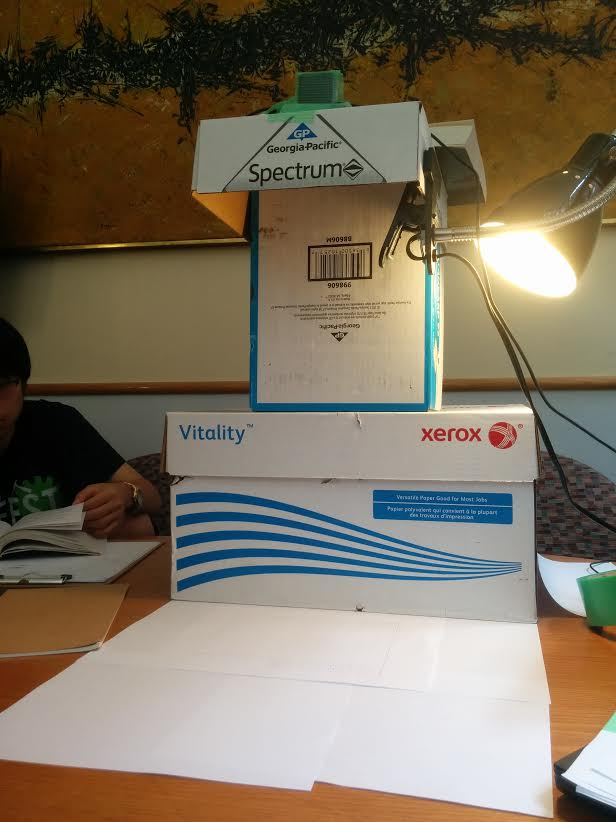
\includegraphics[width=7cm]{device.jpg}};
\begin{scope}[x={7cm / 616},y={-7cm / 616}]
 \draw[red,ultra thick,<-] (350, 90) -- ++(50, 0) node[right,font=\bf\Large] {Camera};
 \draw[red,ultra thick,<-] (520, 320) -- ++(-50, 50) node[below,font=\bf\Large] {Light source};
 \draw[red,ultra thick,<-] (340, 720) node[below,font=\bf\Large] {Paper canvas};
\end{scope}
\end{tikzpicture}

 \caption{The input device}
 \label{fig:1}
\end{figure}
\subsection{Division}
Angus Ding (ad3180) implemented and wrote a report about posture detection, shadow detection and GUI part.
Ayaka Kume (ak3682) implemented and wrote a report about hand detection, fingertip detection and evaluation part.
We wrote introduction and discussion together.
\clearpage
\clearpage
